% !TEX program = xelatex
% Отчет по ПЗ1. Сборка: xelatex report.tex (дважды). Требуются шрифты Times New Roman и Courier New.
% Параметры оформления соответствуют рабочему профилю СТП БГУИР 01-2024:
% A4, поля 30/15/20/20 мм, Times New Roman 14 pt, интервал 18 pt, отступ 1,25 см, латиница курсивом.
\documentclass[14pt,a4paper]{extarticle}
\usepackage{fontspec}
% Times New Roman и Courier New; в Overleaf их нет, поэтому подставляются метрически совместимые TeX Gyre
\IfFontExistsTF{Times New Roman}{\setmainfont{Times New Roman}}{\setmainfont{TeX Gyre Termes}}
\IfFontExistsTF{Courier New}{\setmonofont{Courier New}}{\setmonofont{TeX Gyre Cursor}}
\usepackage{polyglossia}
\setmainlanguage{russian}
\setotherlanguage{english}
\usepackage[a4paper,left=30mm,right=15mm,top=20mm,bottom=20mm]{geometry}
\usepackage{graphicx}
\usepackage{float}
\usepackage{array}
\usepackage{fancyvrb}
\usepackage{enumitem}
\usepackage{titlesec}
\usepackage[labelsep=endash,font=normalsize]{caption}
\usepackage[hidelinks]{hyperref}
\selectlanguage{russian}
\DeclareCaptionLabelFormat{lab}{#1 #2}
\captionsetup[figure]{name=Рисунок,justification=centering,singlelinecheck=false,aboveskip=6pt,belowskip=0pt}
\setlength{\parindent}{1.25cm}
\setlength{\parskip}{0pt}
\setlength{\parfillskip}{0pt plus 1fil}
\renewcommand{\baselinestretch}{1}
\AtBeginDocument{\fontsize{14pt}{18pt}\selectfont}
\sloppy
\newcommand{\LB}{\char123}
\newcommand{\RB}{\char125}
\renewcommand{\thesection}{\arabic{section}}
\renewcommand{\thesubsection}{\arabic{section}.\arabic{subsection}}
\titleformat{\section}{\centering\bfseries\fontsize{14pt}{18pt}\selectfont}{\thesection}{1ex}{}
\titleformat{\subsection}{\bfseries\fontsize{14pt}{18pt}\selectfont}{\hspace{1.25cm}\thesubsection}{1ex}{}
\titlespacing*{\section}{0pt}{18pt}{18pt}
\titlespacing*{\subsection}{0pt}{18pt}{18pt}
\setlist[itemize]{leftmargin=2cm,labelsep=0.75cm,itemsep=0pt,topsep=0pt,parsep=0pt,partopsep=0pt,label=\textbullet}
\setlength{\intextsep}{18pt}
\setlength{\textfloatsep}{18pt}
\begin{document}
\thispagestyle{empty}
{\centering \fontsize{14pt}{18pt}\selectfont Министерство образования Республики Беларусь\par}
{\centering \fontsize{14pt}{18pt}\selectfont Учреждение образования\par}
{\centering \fontsize{14pt}{18pt}\selectfont «Белорусский государственный университет информатики и радиоэлектроники»\par}
\vspace{18pt}
{\centering \fontsize{14pt}{18pt}\selectfont Факультет [УТОЧНИТЬ]\par}
{\centering \fontsize{14pt}{18pt}\selectfont Кафедра [УТОЧНИТЬ]\par}
\vspace{18pt}
\vspace{18pt}
\vspace{18pt}
\vspace{18pt}
{\centering \bfseries \fontsize{16pt}{18pt}\selectfont ОТЧЕТ\par}
{\centering \fontsize{14pt}{18pt}\selectfont по практическому занятию №1\par}
{\centering \fontsize{14pt}{18pt}\selectfont «\textit{Middleware} и шаблонизаторы»\par}
{\centering \fontsize{14pt}{18pt}\selectfont по дисциплине «ИТиВП» [УТОЧНИТЬ полное название]\par}
\vspace{18pt}
\vspace{18pt}
\vspace{18pt}
\vspace{18pt}
\vspace{18pt}
\hspace*{8cm}\parbox[t]{7cm}{\raggedright Выполнил: студент гр. [УТОЧНИТЬ] [УТОЧНИТЬ ФИО]}\par
\hspace*{8cm}\parbox[t]{7cm}{\raggedright Проверил: [УТОЧНИТЬ ФИО преподавателя]}\par
\vspace{18pt}
\vspace{18pt}
\vspace{18pt}
\vspace{18pt}
\vspace{18pt}
{\centering \fontsize{14pt}{18pt}\selectfont Минск 2026\par}
\newpage
\section{Цель работы}

Целью работы является освоение концепции \textit{middleware} в \textit{Express.js}, разработка собственных \textit{middleware} для логирования, имитации авторизации и обработки ошибок, а также изучение шаблонизатора \textit{EJS} для генерации динамических \textit{HTML}-страниц на стороне сервера. Тематика проекта соответствует курсовой работе: платформа для создания визуальных \textit{DSL}-диаграмм (\textit{VisualDSL}), данные которой хранятся в массиве в памяти.

\section{Задание и порядок выполнения}

В рамках практического занятия необходимо решить пять задач, каждая из которых получила отражение в отдельном разделе отчета и в коде проекта:

\begin{itemize}
  \item создать \textit{Express}-приложение с поддержкой \textit{EJS} и настроить \textit{view} \textit{engine}
  \item реализовать \textit{middleware} логирования метода, \textit{URL} и времени запроса с сохранением записей в журнал, который выводится в виде таблицы
  \item реализовать \textit{middleware} имитации авторизации по параметру \textit{?auth=1}
  \item создать динамические страницы: главную, детальную и форму добавления
  \item добавить обработку ошибок 404 и 500 с отдельными страницами
\end{itemize}

Данные хранятся в массиве в оперативной памяти, база данных не используется. Код размещен в ветке \textit{pz21} репозитория проекта.

\section{Ход работы}

Работа выполнена поэтапно: сначала настроены проект и шаблонизатор, затем созданы шаблоны страниц, реализованы \textit{middleware}, маршруты и обработка ошибок, после чего результат проверен в браузере и автоматическими тестами. Каждый этап описан в отдельном подразделе.

\subsection{Настройка проекта и \textit{EJS}}

Проект построен на основе серверной части из предыдущей лабораторной работы: точка входа \textit{server.js} запускает приложение, а само приложение собирается в \textit{app.js}. Такое разделение позволяет подключать приложение в автоматических тестах без запуска сетевого порта. Зависимость \textit{ejs} устанавливается командой \textit{npm install ejs}, а в \textit{app.js} задаются параметры \textit{view engine} и \textit{views} (листинг 1). Статические файлы подключаются до маршрутов, чтобы запросы к стилям не проходили через остальную цепочку \textit{middleware}.

\noindent\vspace{18pt}\par\nopagebreak\noindent Листинг 1 – Настройка \textit{Express} и порядок подключения \textit{middleware} (\textit{app.js})\par\nopagebreak
\begin{Verbatim}[commandchars=\\\{\},fontsize=\small,baselinestretch=1]
\textit{const path = require('path');}
\textit{const express = require('express');}
\textit{const logger = require('./middlewares/logger');}
\textit{const \LB{} attachUser \RB{} = require('./middlewares/auth');}
\textit{const \LB{} notFoundHandler, serverErrorHandler \RB{} = require('./middlewares/errorHandlers');}
\textit{const pageRoutes = require('./routes/pageRoutes');}
\textit{const diagramRoutes = require('./routes/diagramRoutes');}
\textit{ }
\textit{const app = express();}
\textit{ }
\textit{// }Шаблонизатор\textit{ EJS.}
\textit{app.set('view engine', 'ejs');}
\textit{app.set('views', path.join(__dirname, 'views'));}
\textit{ }
\textit{// Helper }для шаблонов\textit{: }форматирование даты\textit{.}
\textit{app.locals.formatDate = (iso) => new Date(iso).toLocaleString('ru-RU');}
\textit{ }
\textit{// }Статика подключается до маршрутов\textit{, }чтобы файлы отдавались без лишних проверок\textit{.}
\textit{app.use('/static', express.static(path.join(__dirname, 'public')));}
\textit{ }
\textit{app.use(logger);}
\textit{ }
\textit{app.use(express.urlencoded(\LB{} extended: true \RB{}));}
\textit{app.use(express.json());}
\textit{app.use(attachUser);}
\textit{ }
\textit{app.use('/', pageRoutes);}
\textit{app.use('/api/diagrams', diagramRoutes);}
\textit{ }
\textit{// }Обработчики ошибок идут последними\textit{.}
\textit{app.use(notFoundHandler);}
\textit{app.use(serverErrorHandler);}
\textit{ }
\textit{module.exports = app;}
\end{Verbatim}
\vspace{18pt}

\subsection{Шаблоны \textit{EJS}}

Общий каркас страницы вынесен в частичные шаблоны \textit{partials/header.ejs} и \textit{partials/footer.ejs}, которые подключаются конструкцией \textit{include} в каждой странице. Благодаря этому разметка \textit{<html>} и шапка сайта не повторяются. Созданы страницы \textit{index.ejs} (список), \textit{item.ejs} (детали), \textit{add.ejs} (форма), \textit{login.ejs}, \textit{404.ejs} и \textit{500.ejs}. Шаблон главной страницы приведен в листинге 2: цикл \textit{forEach} выводит массив диаграмм в таблицу, а вывод через \textit{<\%= \%>} экранирует \textit{HTML}. Шапка сайта, подключаемая во все страницы, приведена в листинге 3.

\noindent\vspace{18pt}\par\nopagebreak\noindent Листинг 2 – Шаблон главной страницы (\textit{views/index.ejs})\par\nopagebreak
\begin{Verbatim}[commandchars=\\\{\},fontsize=\small,baselinestretch=1]
\textit{<%- include('partials/header') %>}
\textit{<h1>}Список диаграмм\textit{</h1>}
\textit{<p><a class="btn" href="/add<%= authQuery %>">}Добавить диаграмму\textit{</a></p>}
\textit{ }
\textit{<% if (items.length === 0) \LB{} %>}
\textit{    <p class="muted">}Диаграмм пока нет\textit{.</p>}
\textit{<% \RB{} else \LB{} %>}
\textit{    <table>}
\textit{        <thead>}
\textit{            <tr><th>ID</th><th>}Название\textit{</th><th>}Тип\textit{</th><th>}Создана\textit{</th></tr>}
\textit{        </thead>}
\textit{        <tbody>}
\textit{            <% items.forEach(function (item) \LB{} %>}
\textit{                <tr>}
\textit{                    <td><%= item.id %></td>}
\textit{                    <td><a href="/item/<%= item.id %><%= authQuery %>"><%= item.title %></a></td>}
\textit{                    <td><span class="badge"><%= item.type %></span></td>}
\textit{                    <td><%= formatDate(item.createdAt) %></td>}
\textit{                </tr>}
\textit{            <% \RB{}); %>}
\textit{        </tbody>}
\textit{    </table>}
\textit{<% \RB{} %>}
\textit{<%- include('partials/footer') %>}
\end{Verbatim}
\vspace{18pt}

\noindent\vspace{18pt}\par\nopagebreak\noindent Листинг 3 – Частичный шаблон шапки (\textit{views/partials/header.ejs})\par\nopagebreak
\begin{Verbatim}[commandchars=\\\{\},fontsize=\small,baselinestretch=1]
\textit{<!DOCTYPE html>}
\textit{<html lang="ru">}
\textit{<head>}
\textit{    <meta charset="UTF-8">}
\textit{    <meta name="viewport" content="width=device-width, initial-scale=1.0">}
\textit{    <title><%= title %> | VisualDSL</title>}
\textit{    <link rel="stylesheet" href="/static/css/style.css">}
\textit{</head>}
\textit{<body>}
\textit{<header class="site-header">}
\textit{    <a class="brand" href="/<%= authQuery %>">VisualDSL</a>}
\textit{    <nav>}
\textit{        <a href="/<%= authQuery %>">}Диаграммы\textit{</a>}
\textit{        <a href="/add<%= authQuery %>">}Добавить\textit{</a>}
\textit{        <a href="/logs<%= authQuery %>">}Журнал\textit{</a>}
\textit{    </nav>}
\textit{    <span class="user">}Пользователь\textit{: <strong><%= user.name %></strong>}
\textit{        <% if (!user.isAuth) \LB{} %><a href="/login">}Войти\textit{</a><% \RB{} %>}
\textit{    </span>}
\textit{</header>}
\textit{<main class="container">}
\end{Verbatim}
\vspace{18pt}

\subsection{\textit{Middleware}}

Логирующее \textit{middleware} (листинг 4) подписывается на событие \textit{finish} ответа, выводит в консоль метод, \textit{URL}, код состояния и время обработки в миллисекундах, а также сохраняет запись в журнал \textit{logStore} (листинг 5). Запись содержит время, тип события (успешный запрос, перенаправление, ошибка клиента или сервера), метод, \textit{URL}, статус, длительность, имя пользователя и \textit{IP}-адрес; журнал ограничен 500 записями и выводится таблицей на странице \textit{/logs}. \textit{Middleware} авторизации (листинг 6) состоит из двух функций: \textit{attachUser} определяет пользователя по параметру \textit{?auth=1} и передает его в шаблоны через \textit{res.locals}, а \textit{requireAuth} перенаправляет гостя на \textit{/login}. Обе стратегии, допустимые заданием, реализованы одновременно: гость получает \textit{req.user} со значением «Гость», а защищенные маршруты требуют авторизацию.

\noindent\vspace{18pt}\par\nopagebreak\noindent Листинг 4 – \textit{Middleware} логирования (\textit{middlewares/logger.js})\par\nopagebreak
\begin{Verbatim}[commandchars=\\\{\},fontsize=\small,baselinestretch=1]
\textit{// }Логирование\textit{: }метод\textit{, URL, }статус и время обработки\textit{ (}мс\textit{) }после отправки ответа\textit{.}
\textit{// }Запись попадает в журнал\textit{ (}таблица на странице\textit{ /logs) }и в консоль\textit{ (}кроме тестов\textit{).}
\textit{const logStore = require('../models/logStore');}
\textit{ }
\textit{module.exports = (req, res, next) => \LB{}}
\textit{  const start = process.hrtime.bigint();}
\textit{ }
\textit{  res.on('finish', () => \LB{}}
\textit{    const ms = Number(process.hrtime.bigint() - start) / 1e6;}
\textit{    const entry = logStore.add(\LB{}}
\textit{      method: req.method,}
\textit{      url: req.originalUrl,}
\textit{      status: res.statusCode,}
\textit{      durationMs: ms,}
\textit{      user: req.user ? req.user.name : '}Гость\textit{',}
\textit{      ip: req.ip || '-'}
\textit{    \RB{});}
\textit{ }
\textit{    if (process.env.NODE_ENV !== 'test') \LB{}}
\textit{      console.log(}
\textit{        `[$\LB{}entry.time\RB{}] $\LB{}entry.method\RB{} $\LB{}entry.url\RB{} -> $\LB{}entry.status\RB{} ($\LB{}entry.durationMs.toFixed(2)\RB{} }мс\textit{)`}
\textit{      );}
\textit{    \RB{}}
\textit{  \RB{});}
\textit{ }
\textit{  next();}
\textit{\RB{};}
\end{Verbatim}
\vspace{18pt}

\noindent\vspace{18pt}\par\nopagebreak\noindent Листинг 5 – Хранилище журнала запросов (\textit{models/logStore.js})\par\nopagebreak
\begin{Verbatim}[commandchars=\\\{\},fontsize=\small,baselinestretch=1]
\textit{// }Журнал запросов в памяти\textit{: }записи отображаются на странице\textit{ /logs }в виде таблицы\textit{.}
\textit{const MAX_ENTRIES = 500;}
\textit{ }
\textit{let entries = [];}
\textit{let nextId = 1;}
\textit{ }
\textit{// }Тип события определяется по коду ответа\textit{.}
\textit{const eventByStatus = (status) => \LB{}}
\textit{  if (status >= 500) return '}Ошибка сервера\textit{';}
\textit{  if (status >= 400) return '}Ошибка клиента\textit{';}
\textit{  if (status >= 300) return '}Перенаправление\textit{';}
\textit{  return '}Успешный запрос\textit{';}
\textit{\RB{};}
\textit{ }
\textit{const add = (\LB{} method, url, status, durationMs, user, ip \RB{}) => \LB{}}
\textit{  const entry = \LB{}}
\textit{    id: nextId++,}
\textit{    time: new Date().toISOString(),}
\textit{    event: eventByStatus(status),}
\textit{    method,}
\textit{    url,}
\textit{    status,}
\textit{    durationMs: Number(durationMs.toFixed(2)),}
\textit{    user,}
\textit{    ip}
\textit{  \RB{};}
\textit{  entries.push(entry);}
\textit{  if (entries.length > MAX_ENTRIES) entries.shift();}
\textit{  return entry;}
\textit{\RB{};}
\textit{ }
\textit{// }Новые записи первыми\textit{; }необязательные фильтры по методу и классу события\textit{.}
\textit{const getAll = (\LB{} method, event \RB{} = \LB{}\RB{}) =>}
\textit{  entries}
\textit{    .filter((e) => (!method || e.method === method) && (!event || e.event === event))}
\textit{    .reverse();}
\textit{ }
\textit{const clear = () => \LB{}}
\textit{  entries = [];}
\textit{  nextId = 1;}
\textit{\RB{};}
\textit{ }
\textit{module.exports = \LB{} MAX_ENTRIES, eventByStatus, add, getAll, clear \RB{};}
\end{Verbatim}
\vspace{18pt}

\noindent\vspace{18pt}\par\nopagebreak\noindent Листинг 6 – \textit{Middleware} имитации авторизации (\textit{middlewares/auth.js})\par\nopagebreak
\begin{Verbatim}[commandchars=\\\{\},fontsize=\small,baselinestretch=1]
\textit{// }Имитация авторизации по\textit{ query-}параметру\textit{ ?auth=1 (}без сессий и паролей\textit{).}
\textit{const GUEST = \LB{} name: '}Гость\textit{', isAuth: false \RB{};}
\textit{const ADMIN = \LB{} name: '}Администратор\textit{', isAuth: true \RB{};}
\textit{ }
\textit{// }Определяет пользователя и передает его в шаблоны\textit{ (res.locals).}
\textit{const attachUser = (req, res, next) => \LB{}}
\textit{  req.user = req.query.auth === '1' ? ADMIN : GUEST;}
\textit{  res.locals.user = req.user;}
\textit{  // }Суффикс для ссылок\textit{, }чтобы\textit{ "}авторизация\textit{" }сохранялась при переходах по сайту\textit{.}
\textit{  res.locals.authQuery = req.user.isAuth ? '?auth=1' : '';}
\textit{  next();}
\textit{\RB{};}
\textit{ }
\textit{// }Защита маршрута\textit{: }гость перенаправляется на\textit{ /login.}
\textit{const requireAuth = (req, res, next) => \LB{}}
\textit{  if (req.user && req.user.isAuth) return next();}
\textit{  res.redirect('/login');}
\textit{\RB{};}
\textit{ }
\textit{module.exports = \LB{} attachUser, requireAuth \RB{};}
\end{Verbatim}
\vspace{18pt}

\subsection{Маршруты и рендеринг}

Маршруты страниц описаны в \textit{routes/pageRoutes.js} (листинг 7), а логика обработчиков находится в \textit{controllers/pageController.js}. Список и детальная страница доступны всем, маршруты \textit{/add} защищены \textit{middleware} \textit{requireAuth}. Данные берутся из общего хранилища \textit{models/diagramStore.js}, которое используется и страницами, и \textit{REST} \textit{API}, поэтому добавленная через форму диаграмма сразу видна в \textit{API}. Форма проверяет поля на стороне сервера и при ошибке повторно показывает введенные значения с кодом 400.

\noindent\vspace{18pt}\par\nopagebreak\noindent Листинг 7 – Маршруты страниц (\textit{routes/pageRoutes.js})\par\nopagebreak
\begin{Verbatim}[commandchars=\\\{\},fontsize=\small,baselinestretch=1]
\textit{const express = require('express');}
\textit{const \LB{} requireAuth \RB{} = require('../middlewares/auth');}
\textit{const pages = require('../controllers/pageController');}
\textit{ }
\textit{const router = express.Router();}
\textit{ }
\textit{router.get('/', pages.index);}
\textit{router.get('/item/:id', pages.item);}
\textit{router.get('/login', pages.login);}
\textit{router.get('/logs', pages.logs);}
\textit{// Middleware requireAuth }выполняется только для этих маршрутов\textit{.}
\textit{router.get('/add', requireAuth, pages.addForm);}
\textit{router.post('/add', requireAuth, pages.addSubmit);}
\textit{ }
\textit{if (process.env.NODE_ENV !== 'production') \LB{}}
\textit{  router.get('/debug/error', pages.crash);}
\textit{\RB{}}
\textit{ }
\textit{module.exports = router;}
\end{Verbatim}
\vspace{18pt}

\subsection{Обработка ошибок}

Обработчики ошибок (листинг 8) подключаются последними. Функция \textit{notFoundHandler} отображает страницу \textit{404.ejs}, а \textit{serverErrorHandler} имеет четыре параметра, что делает ее обработчиком ошибок \textit{Express}: она пишет стек в консоль и отображает \textit{500.ejs}. Для запросов к \textit{/api/} обе функции возвращают \textit{JSON}, поэтому клиенты \textit{API} не получают \textit{HTML}. Для демонстрации страницы 500 добавлен маршрут \textit{/debug/error}, отключаемый при \textit{NODE\_ENV=production}.

\noindent\vspace{18pt}\par\nopagebreak\noindent Листинг 8 – Обработчики ошибок (\textit{middlewares/errorHandlers.js})\par\nopagebreak
\begin{Verbatim}[commandchars=\\\{\},fontsize=\small,baselinestretch=1]
\textit{// }Обработчики ошибок\textit{: 404 (}маршрут не найден\textit{) }и\textit{ 500 (}исключение в приложении\textit{).}
\textit{const wantsJson = (req) => req.originalUrl.startsWith('/api/');}
\textit{ }
\textit{const notFoundHandler = (req, res) => \LB{}}
\textit{  if (wantsJson(req)) return res.status(404).json(\LB{} error: '}Маршрут не найден\textit{' \RB{});}
\textit{  res.status(404).render('404', \LB{} title: '}Ошибка\textit{ 404' \RB{});}
\textit{\RB{};}
\textit{ }
\textit{// }Четыре параметра\textit{ - }признак\textit{ error-handling middleware }в\textit{ Express.}
\textit{const serverErrorHandler = (err, req, res, next) => \LB{}}
\textit{  console.error(err.stack || err);}
\textit{  if (res.headersSent) return next(err);}
\textit{  if (wantsJson(req)) \LB{}}
\textit{    return res.status(500).json(\LB{} error: '}Внутренняя ошибка сервера\textit{', message: err.message \RB{});}
\textit{  \RB{}}
\textit{  res.status(500).render('500', \LB{} title: '}Ошибка\textit{ 500' \RB{});}
\textit{\RB{};}
\textit{ }
\textit{module.exports = \LB{} notFoundHandler, serverErrorHandler \RB{};}
\end{Verbatim}
\vspace{18pt}

\subsection{Результаты работы приложения}

Для проверки приложение запущено командой \textit{npm start}, страницы открыты в браузере. Главная страница с таблицей диаграмм из массива показана на рисунке 1.

\begin{figure}[H]
  \centering
  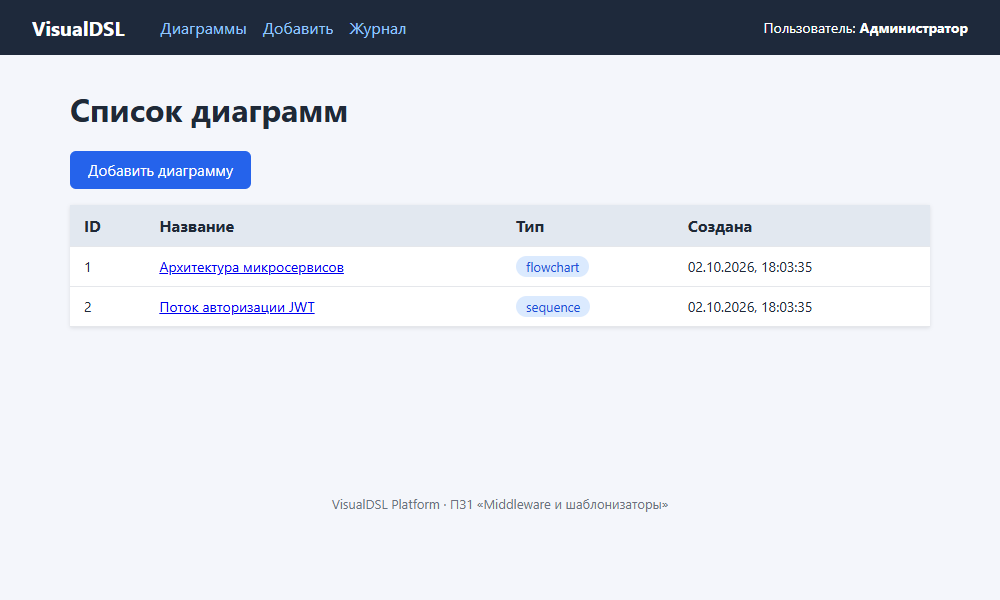
\includegraphics[width=14.5cm]{../screenshots/01-index.png}
  \caption{Главная страница со списком диаграмм}
\end{figure}

На рисунке 1 видны два начальных элемента массива, а имя пользователя в шапке и параметр \textit{?auth=1} в ссылках подтверждают работу \textit{middleware} авторизации. Цикл \textit{forEach} в шаблоне \textit{index.ejs} вывел каждый элемент отдельной строкой таблицы.

Страница на рисунке 2 открывается по адресу \textit{/item/1} и выводит поля выбранного элемента.

\begin{figure}[H]
  \centering
  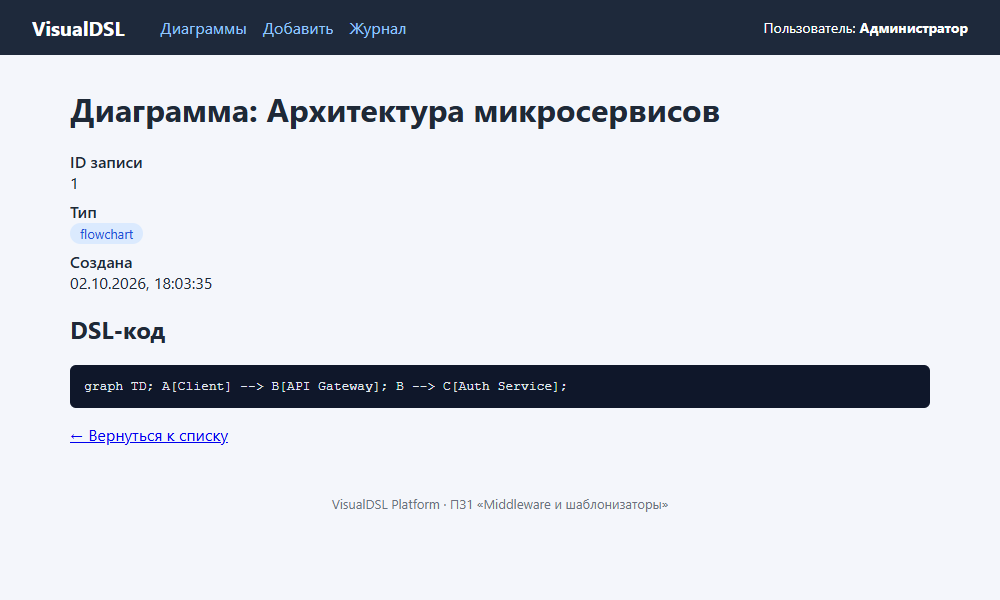
\includegraphics[width=14.5cm]{../screenshots/02-item.png}
  \caption{Детальная страница диаграммы}
\end{figure}

Маршрут \textit{/item/:id} нашел элемент по идентификатору и передал его в шаблон \textit{item.ejs}. \textit{DSL}-код отображается в экранированном виде, поэтому разметка внутри кода не может выполниться в браузере.

Форма добавления доступна только после авторизации и показана на рисунке 3.

\begin{figure}[H]
  \centering
  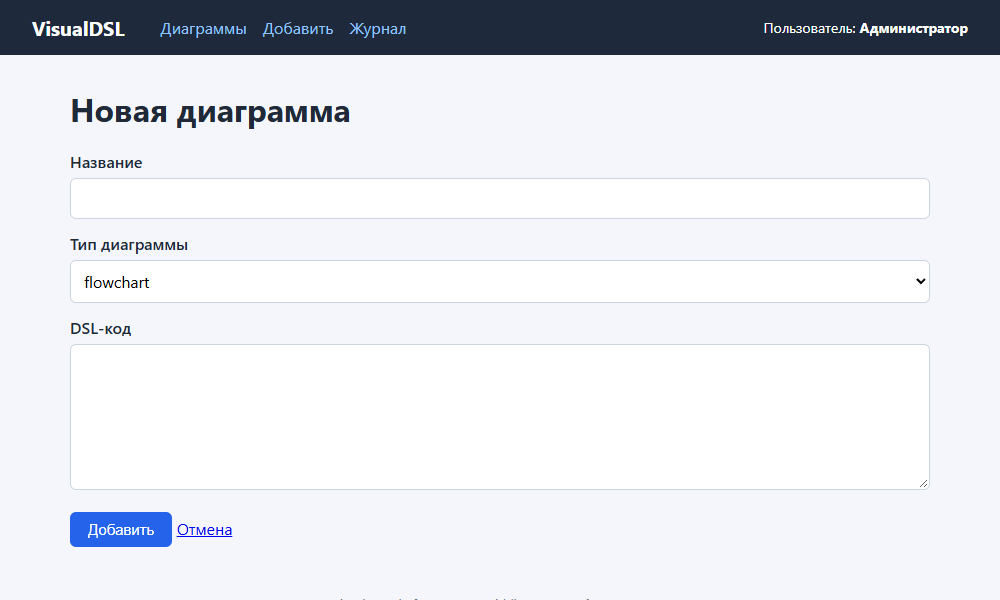
\includegraphics[width=14.5cm]{../screenshots/03-add-form.png}
  \caption{Форма добавления диаграммы}
\end{figure}

Форма содержит поля названия, типа и \textit{DSL}-кода. Адрес отправки \textit{/add?auth=1} сохраняет признак авторизации, поэтому после отправки пользователь остается в системе.

Заполненная форма с данными новой диаграммы приведена на рисунке 4.

\begin{figure}[H]
  \centering
  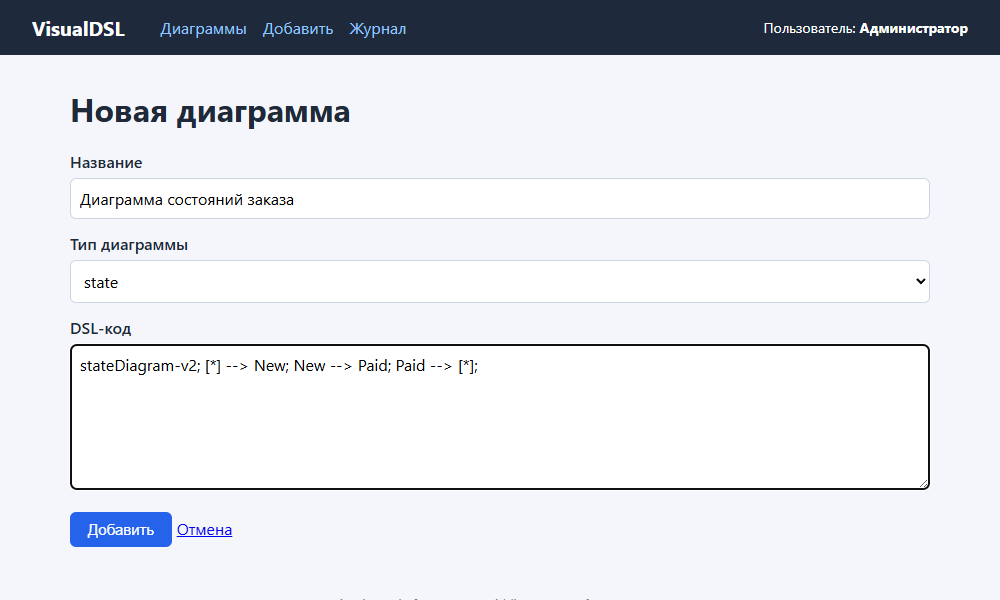
\includegraphics[width=14.5cm]{../screenshots/04-add-form-filled.png}
  \caption{Заполненная форма}
\end{figure}

Введены название «Диаграмма состояний заказа», тип \textit{state} и \textit{DSL}-код. После нажатия кнопки данные уходят методом \textit{POST} на сервер, где проходят проверку.

Результат отправки показан на рисунке 5: сервер выполнил перенаправление на главную страницу.

\begin{figure}[H]
  \centering
  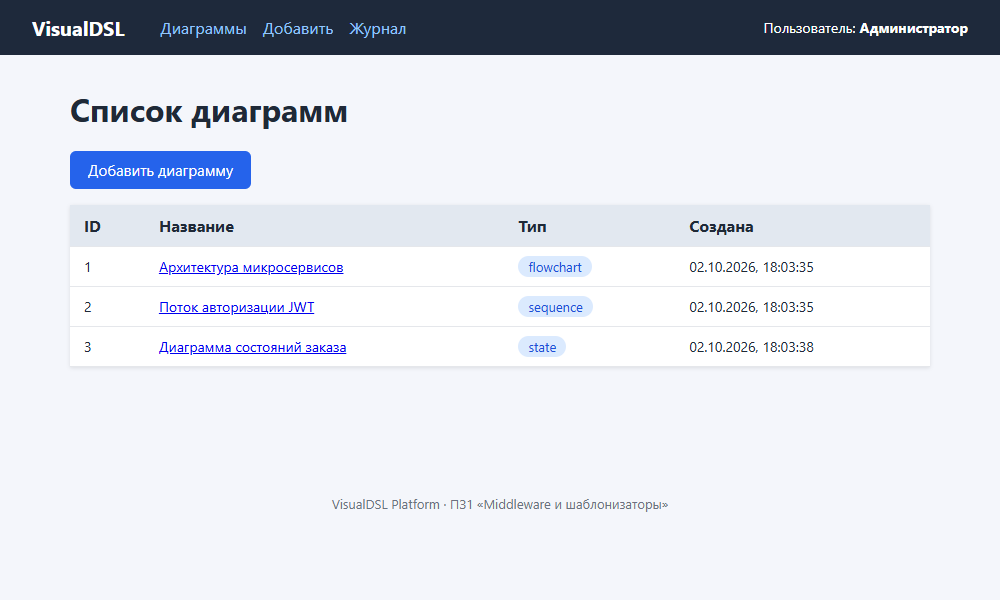
\includegraphics[width=14.5cm]{../screenshots/05-index-after-add.png}
  \caption{Список после добавления элемента}
\end{figure}

Новая диаграмма появилась в списке третьей строкой. Это подтверждает, что \textit{POST /add} добавил элемент в массив, а перенаправление исключает повторную отправку формы при обновлении страницы.

При отправке пустой формы сервер отвечает кодом 400 и показывает список ошибок (рисунок 6).

\begin{figure}[H]
  \centering
  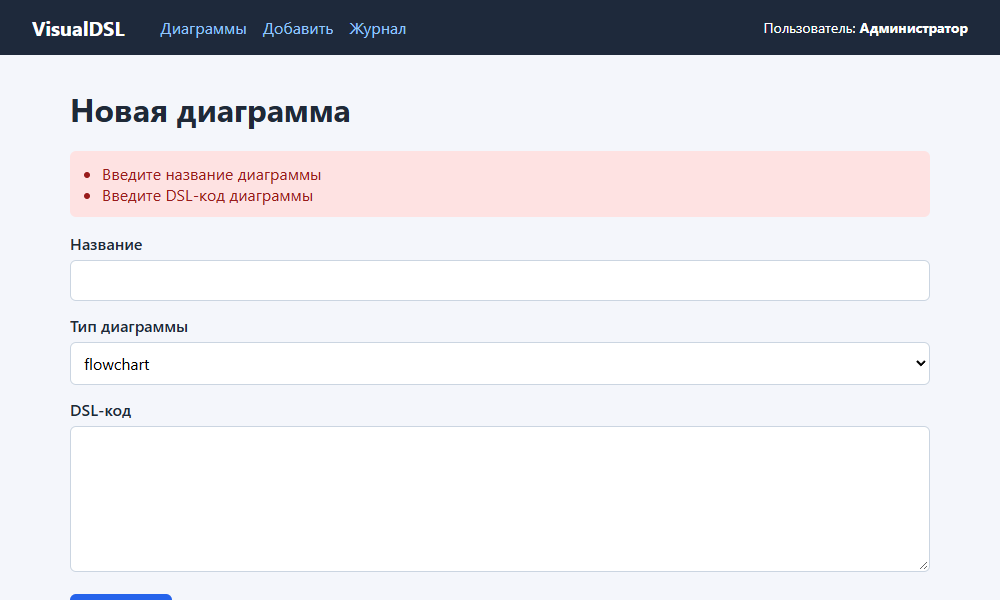
\includegraphics[width=14.5cm]{../screenshots/06-add-validation.png}
  \caption{Сообщения валидации формы}
\end{figure}

Проверка выполняется на стороне сервера: пустые поля названия и \textit{DSL}-кода отклонены, а введенные значения сохранены в форме. Массив данных при этом не изменился.

Гость, открывший \textit{/add} без параметра \textit{auth}, попадает на страницу \textit{/login} (рисунок 7).

\begin{figure}[H]
  \centering
  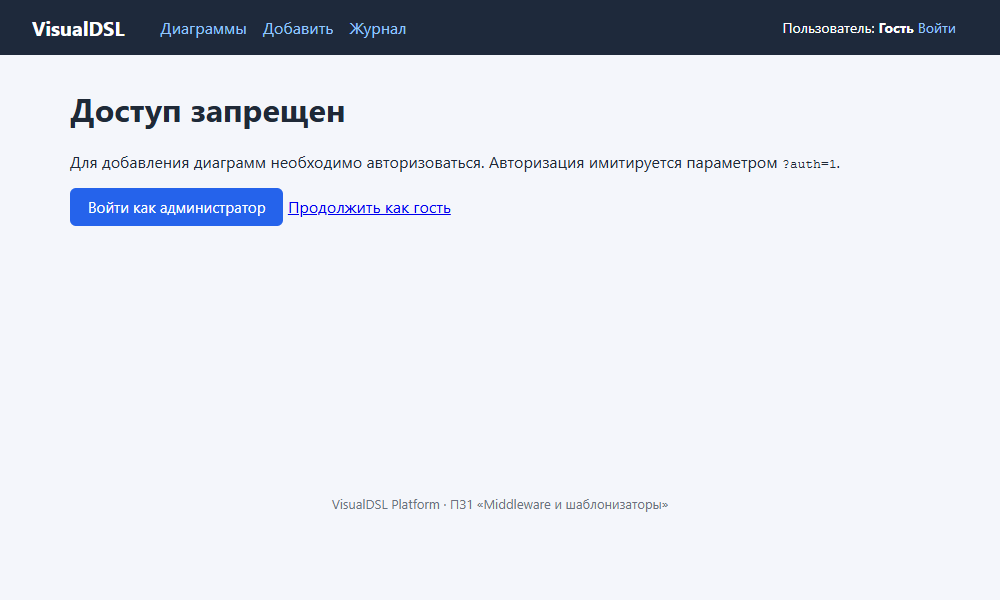
\includegraphics[width=14.5cm]{../screenshots/07-login-redirect.png}
  \caption{Перенаправление гостя на страницу авторизации}
\end{figure}

\textit{Middleware} \textit{requireAuth} остановил запрос и выполнил перенаправление. Страница предлагает войти как администратор через \textit{?auth=1} или продолжить как гость.

Несуществующий адрес приводит к странице 404 (рисунок 8).

\begin{figure}[H]
  \centering
  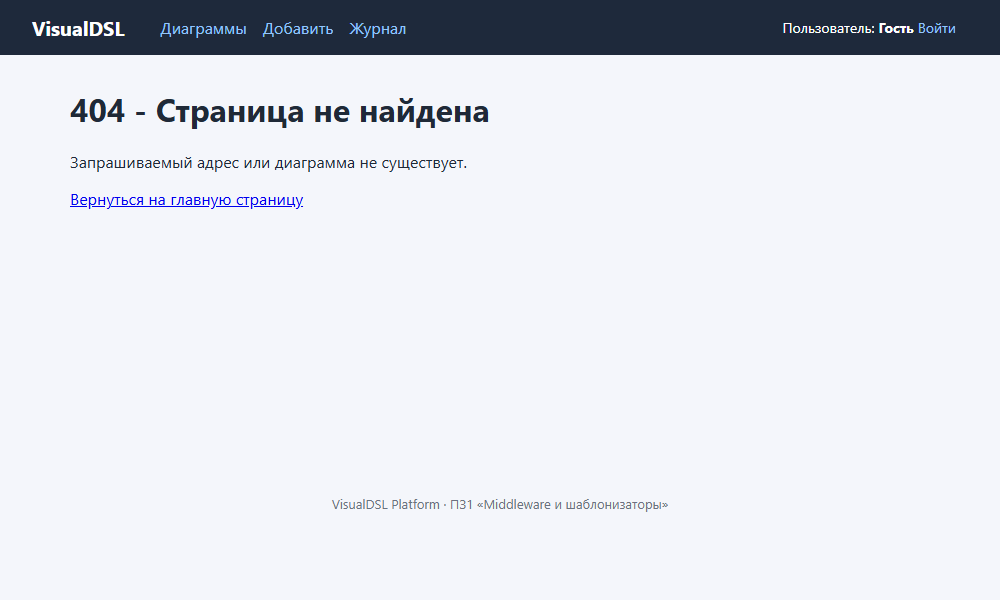
\includegraphics[width=14.5cm]{../screenshots/08-404.png}
  \caption{Страница ошибки 404}
\end{figure}

Обработчик \textit{notFoundHandler} сработал, потому что ни один маршрут не ответил на запрос, и отобразил отдельный шаблон \textit{404.ejs} с ссылкой на главную страницу.

Намеренно вызванное исключение на маршруте \textit{/debug/error} приводит к странице 500 (рисунок 9).

\begin{figure}[H]
  \centering
  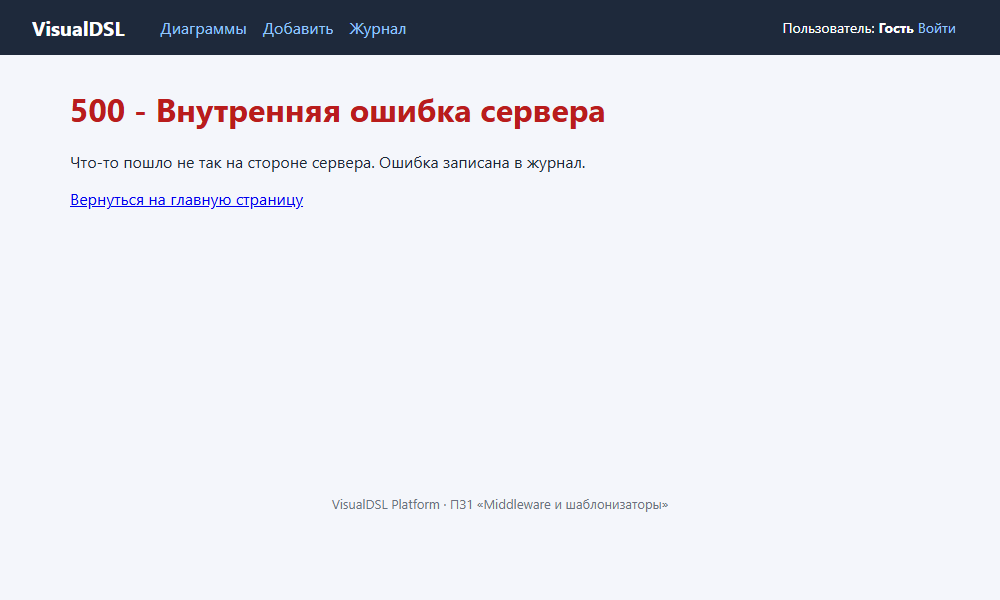
\includegraphics[width=14.5cm]{../screenshots/09-500.png}
  \caption{Страница ошибки 500}
\end{figure}

Обработчик ошибок \textit{serverErrorHandler} записал стек в консоль и показал пользователю безопасную страницу \textit{500.ejs} без технических подробностей.

Журнал запросов, сохраненный логирующим \textit{middleware}, показан таблицей на странице \textit{/logs} (рисунок 10).

\begin{figure}[H]
  \centering
  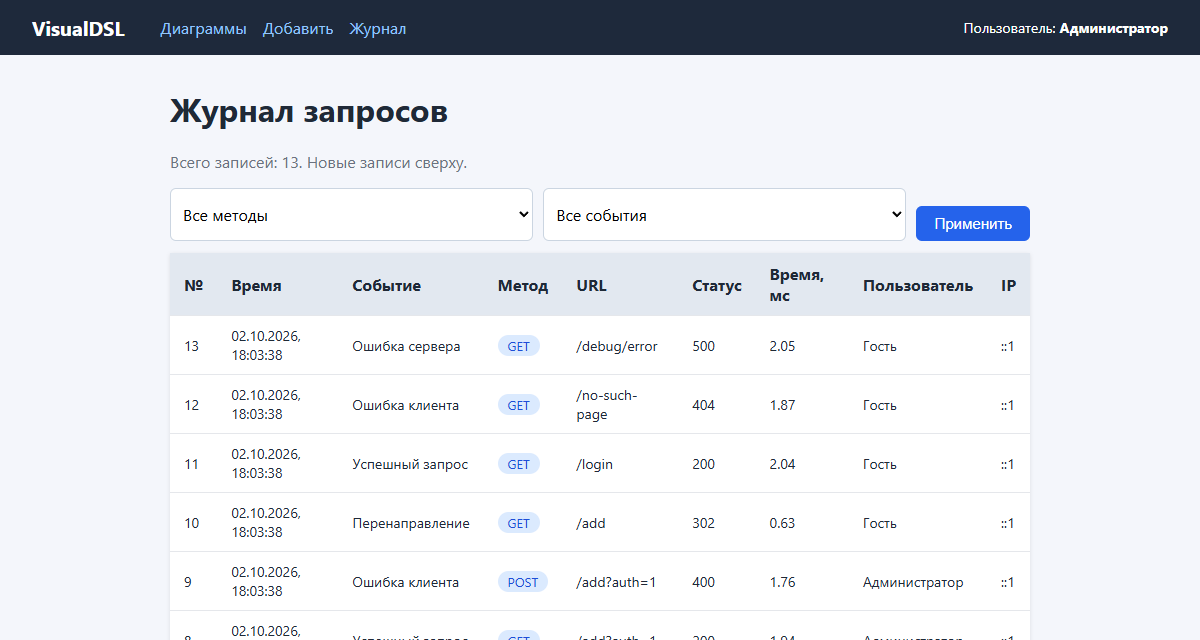
\includegraphics[width=14.5cm]{../screenshots/10-logs-table.png}
  \caption{Журнал запросов в виде таблицы (страница \textit{/logs})}
\end{figure}

В таблице видны время, событие, метод, \textit{URL}, статус, длительность, пользователь и \textit{IP}-адрес. Запросы разных видов отличаются типом события: успешный запрос, перенаправление, ошибка клиента и ошибка сервера. Новые записи расположены сверху.

Таблицу можно отфильтровать по методу и типу события; на рисунке 11 оставлены только запросы \textit{POST}.

\begin{figure}[H]
  \centering
  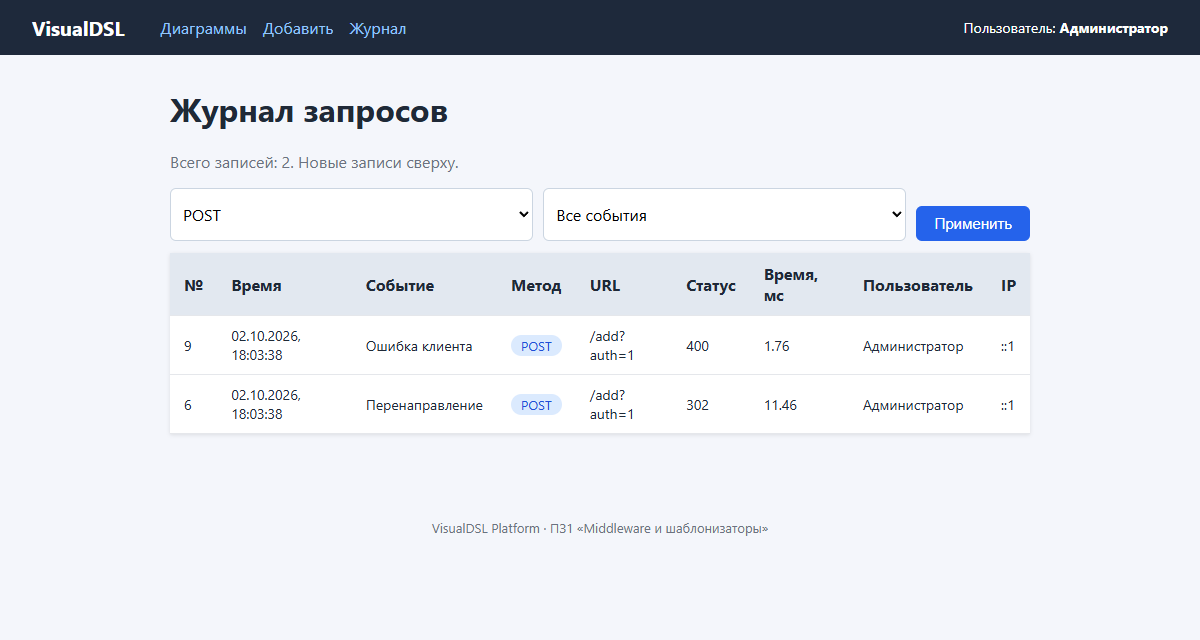
\includegraphics[width=14.5cm]{../screenshots/11-logs-filter.png}
  \caption{Журнал с фильтром по методу \textit{POST}}
\end{figure}

Фильтр передается параметрами строки запроса, а сервер проверяет их по списку допустимых значений, поэтому произвольный ввод игнорируется.

Те же записи выводятся в консоль сервера (рисунок 12), что удобно при отладке.

\begin{figure}[H]
  \centering
  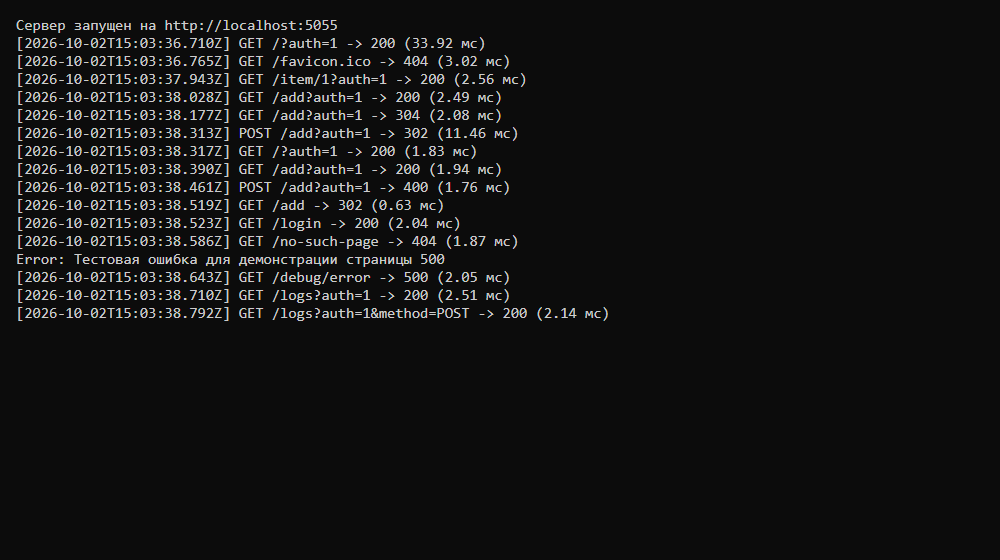
\includegraphics[width=14.5cm]{../screenshots/12-console-log.png}
  \caption{Журнал запросов в консоли сервера}
\end{figure}

Каждая строка содержит время, метод, \textit{URL}, код ответа и длительность обработки в миллисекундах. Сообщение «\textit{Error}» перед последней строкой появилось при обращении к \textit{/debug/error} и подтверждает, что ошибка сервера записывается в журнал.

\subsection{Автоматическое тестирование}

Для проверки приложения написаны автоматические тесты на \textit{Jest} и \textit{Supertest}. Они вызывают приложение без запуска сервера и проверяют коды ответов, содержимое \textit{HTML}, редиректы, экранирование и работу каждого \textit{middleware} по отдельности. Результаты приведены в таблице 1; команда запуска: \textit{npm test}.

\noindent\vspace{18pt}\par\nopagebreak\noindent Таблица 1 – Результаты автоматического тестирования\par\nopagebreak
{\fontsize{12pt}{14pt}\selectfont\setlength{\tabcolsep}{2pt}
\begin{center}\begin{tabular}{|>{\centering\arraybackslash}m{45mm}|>{\centering\arraybackslash}m{95mm}|>{\centering\arraybackslash}m{25mm}|}\hline
\textbf{Набор тестов} & \textbf{Что проверяется} & \textbf{Тестов} \\ \hline
\textit{api.test.js} & \textit{REST} \textit{API} \textit{/api/diagrams}: \textit{CRUD}, поиск, валидация, \textit{JSON}-ошибки & 25 \\ \hline
\textit{pages.test.js} & \textit{EJS}-страницы, авторизация, форма, журнал \textit{/logs}, 404 и 500, статика, \textit{XSS} & 30 \\ \hline
\textit{middleware.test.js} & \textit{logger}, \textit{logStore}, \textit{attachUser}, \textit{requireAuth}, обработчики ошибок, хранилище & 21 \\ \hline
\textit{seeds.test.js} & Начальные данные, фильтры журнала, \textit{production}, запуск \textit{server.js}, сквозной сценарий & 14 \\ \hline
\textit{branches.test.js} & Редкие ветви: пустое тело запроса, ошибка без стека & 5 \\ \hline
\textit{extras/\_\_tests\_\_} & Заготовки для защиты: блокировка \textit{IP}, \textit{CSRF}, поиск, редактирование и другие & 14 \\ \hline
\textit{src/\_\_tests\_\_} & Тесты \textit{React}-компонентов предыдущих работ & 8 \\ \hline
Итого & Все наборы пройдены успешно & 117 \\ \hline
\end{tabular}\end{center}}
\vspace{18pt}

Покрытие серверного кода, измеренное командой \textit{npm run test:coverage}, составило 100 \% по строкам, функциям и операторам и 96,5 \% по ветвям. Непокрытыми остаются только запасные выражения \textit{req.body || \{\}}, которые недостижимы, так как парсеры \textit{Express} всегда создают объект \textit{req.body}. Начальные данные для тестов и демонстрации вынесены в папку \textit{seeds/}: массив диаграмм и набор записей журнала, содержащий все типы событий и методы. Для показа на защите добавлена команда \textit{npm run demo}, которая отправляет на запущенный сервер запросы всех видов и наполняет таблицу журнала.

\section{Ответы на контрольные вопросы}

{\noindent\hspace*{1.25cm}\bfseries 25. Как реализовать защиту от \textit{CSRF} с помощью \textit{middleware} (теоретически)?\par}\nopagebreak
Сервер выдает случайный токен, сохраняет его в сессии и вставляет скрытым полем в форму. \textit{Middleware} сравнивает токен из тела запроса с сохраненным и отклоняет запрос при несовпадении. Дополнительно используют \textit{cookie} с \textit{SameSite}. Готовое решение – пакет \textit{csurf} или его аналоги.

{\noindent\hspace*{1.25cm}\bfseries 26. Как в \textit{EJS} использовать функцию-\textit{helper}?\par}\nopagebreak
Функцию кладут в \textit{app.locals}: \textit{app.locals.formatDate = (iso) => new Date(iso).toLocaleString('ru-RU')}. В шаблоне ее вызывают как обычную: \textit{<\%= formatDate(item.createdAt) \%>}. В проекте так сделано на главной и детальной страницах.

{\noindent\hspace*{1.25cm}\bfseries 27. Почему \textit{middleware} для статики обычно подключается до всех маршрутов?\par}\nopagebreak
Запросы к стилям, скриптам и картинкам должны обслуживаться сразу, не проходя через авторизацию, парсеры и логику маршрутов. Это ускоряет ответ и исключает случайный перехват файлов обработчиком 404.

\section{Выводы}

В ходе работы создано \textit{Express}-приложение с шаблонизатором \textit{EJS}, тематика которого соответствует проекту \textit{VisualDSL}. Реализованы \textit{middleware} логирования с выводом журнала в таблицу (время, событие, метод, \textit{URL}, статус и другие поля) и имитации авторизации, страницы списка, деталей и добавления элемента, а также отдельные страницы ошибок 404 и 500. Данные хранятся в массиве в памяти и используются как \textit{HTML}-страницами, так и \textit{REST} \textit{API}.

Правильность работы подтверждена 117 автоматическими тестами и скриншотами страниц, а покрытие серверного кода по строкам составило 100 \%. Практическим результатом стало понимание того, что порядок подключения \textit{middleware} определяет поведение приложения: статика и разбор тела запроса подключаются до маршрутов, а обработчики 404 и 500 – после них.

\end{document}
